\documentclass[12pt,openright,twoside,a4paper,english,spanish]{abntex2}

\usepackage{cmap}
\usepackage{lmodern}
\usepackage[T1]{fontenc}
\usepackage[utf8]{inputenc}
\usepackage{lastpage}
\usepackage{indentfirst}
\usepackage{color}
\usepackage{graphicx}
\usepackage{units}
\usepackage[brazilian,hyperpageref]{backref}
\usepackage[alf]{abntex2cite}
\usepackage{bold-extra}
\usepackage{eso-pic}
\usepackage{hyperref}
\usepackage{booktabs}
\usepackage{longtable}
\usepackage{multicol}
\renewcommand{\backrefpagesname}{Citado na(s) página(s):~}
\renewcommand{\backref}{}
\renewcommand*{\backrefalt}[4]{
	\ifcase #1 %
		Nenhuma citação no texto.%
	\or
		Citado na página #2.%
	\else
		Citado #1 vezes nas páginas #2.%
	\fi}%
% ---


\newcommand{\curso}[1]{\def\imprimircurso{#1}}

\newcommand{\palavraChaveUm}[1]{\def\imprimirpalavrachaveum{#1}}
\newcommand{\palavraChaveDois}[1]{\def\imprimirpalavrachavedois{#1}}

\newcommand{\cdu}[1]{\def\nomecdu{#1}}
\newcommand{\dataDaAprovacao}[1]{\def\imprimirdatadaaprovacao{#1}}

\newcommand{\membroConvidadoUm}[1]{\def\imprimirmembroconvidadoum{#1}}
\newcommand{\membroConvidadoDois}[1]{\def\imprimirmembroconvidadodois{#1}}

\newcommand\BackgroundPic{%
	\put(0,0){%
		\parbox[b][\paperheight]{\paperwidth}{%
			\vfill
			\centering
			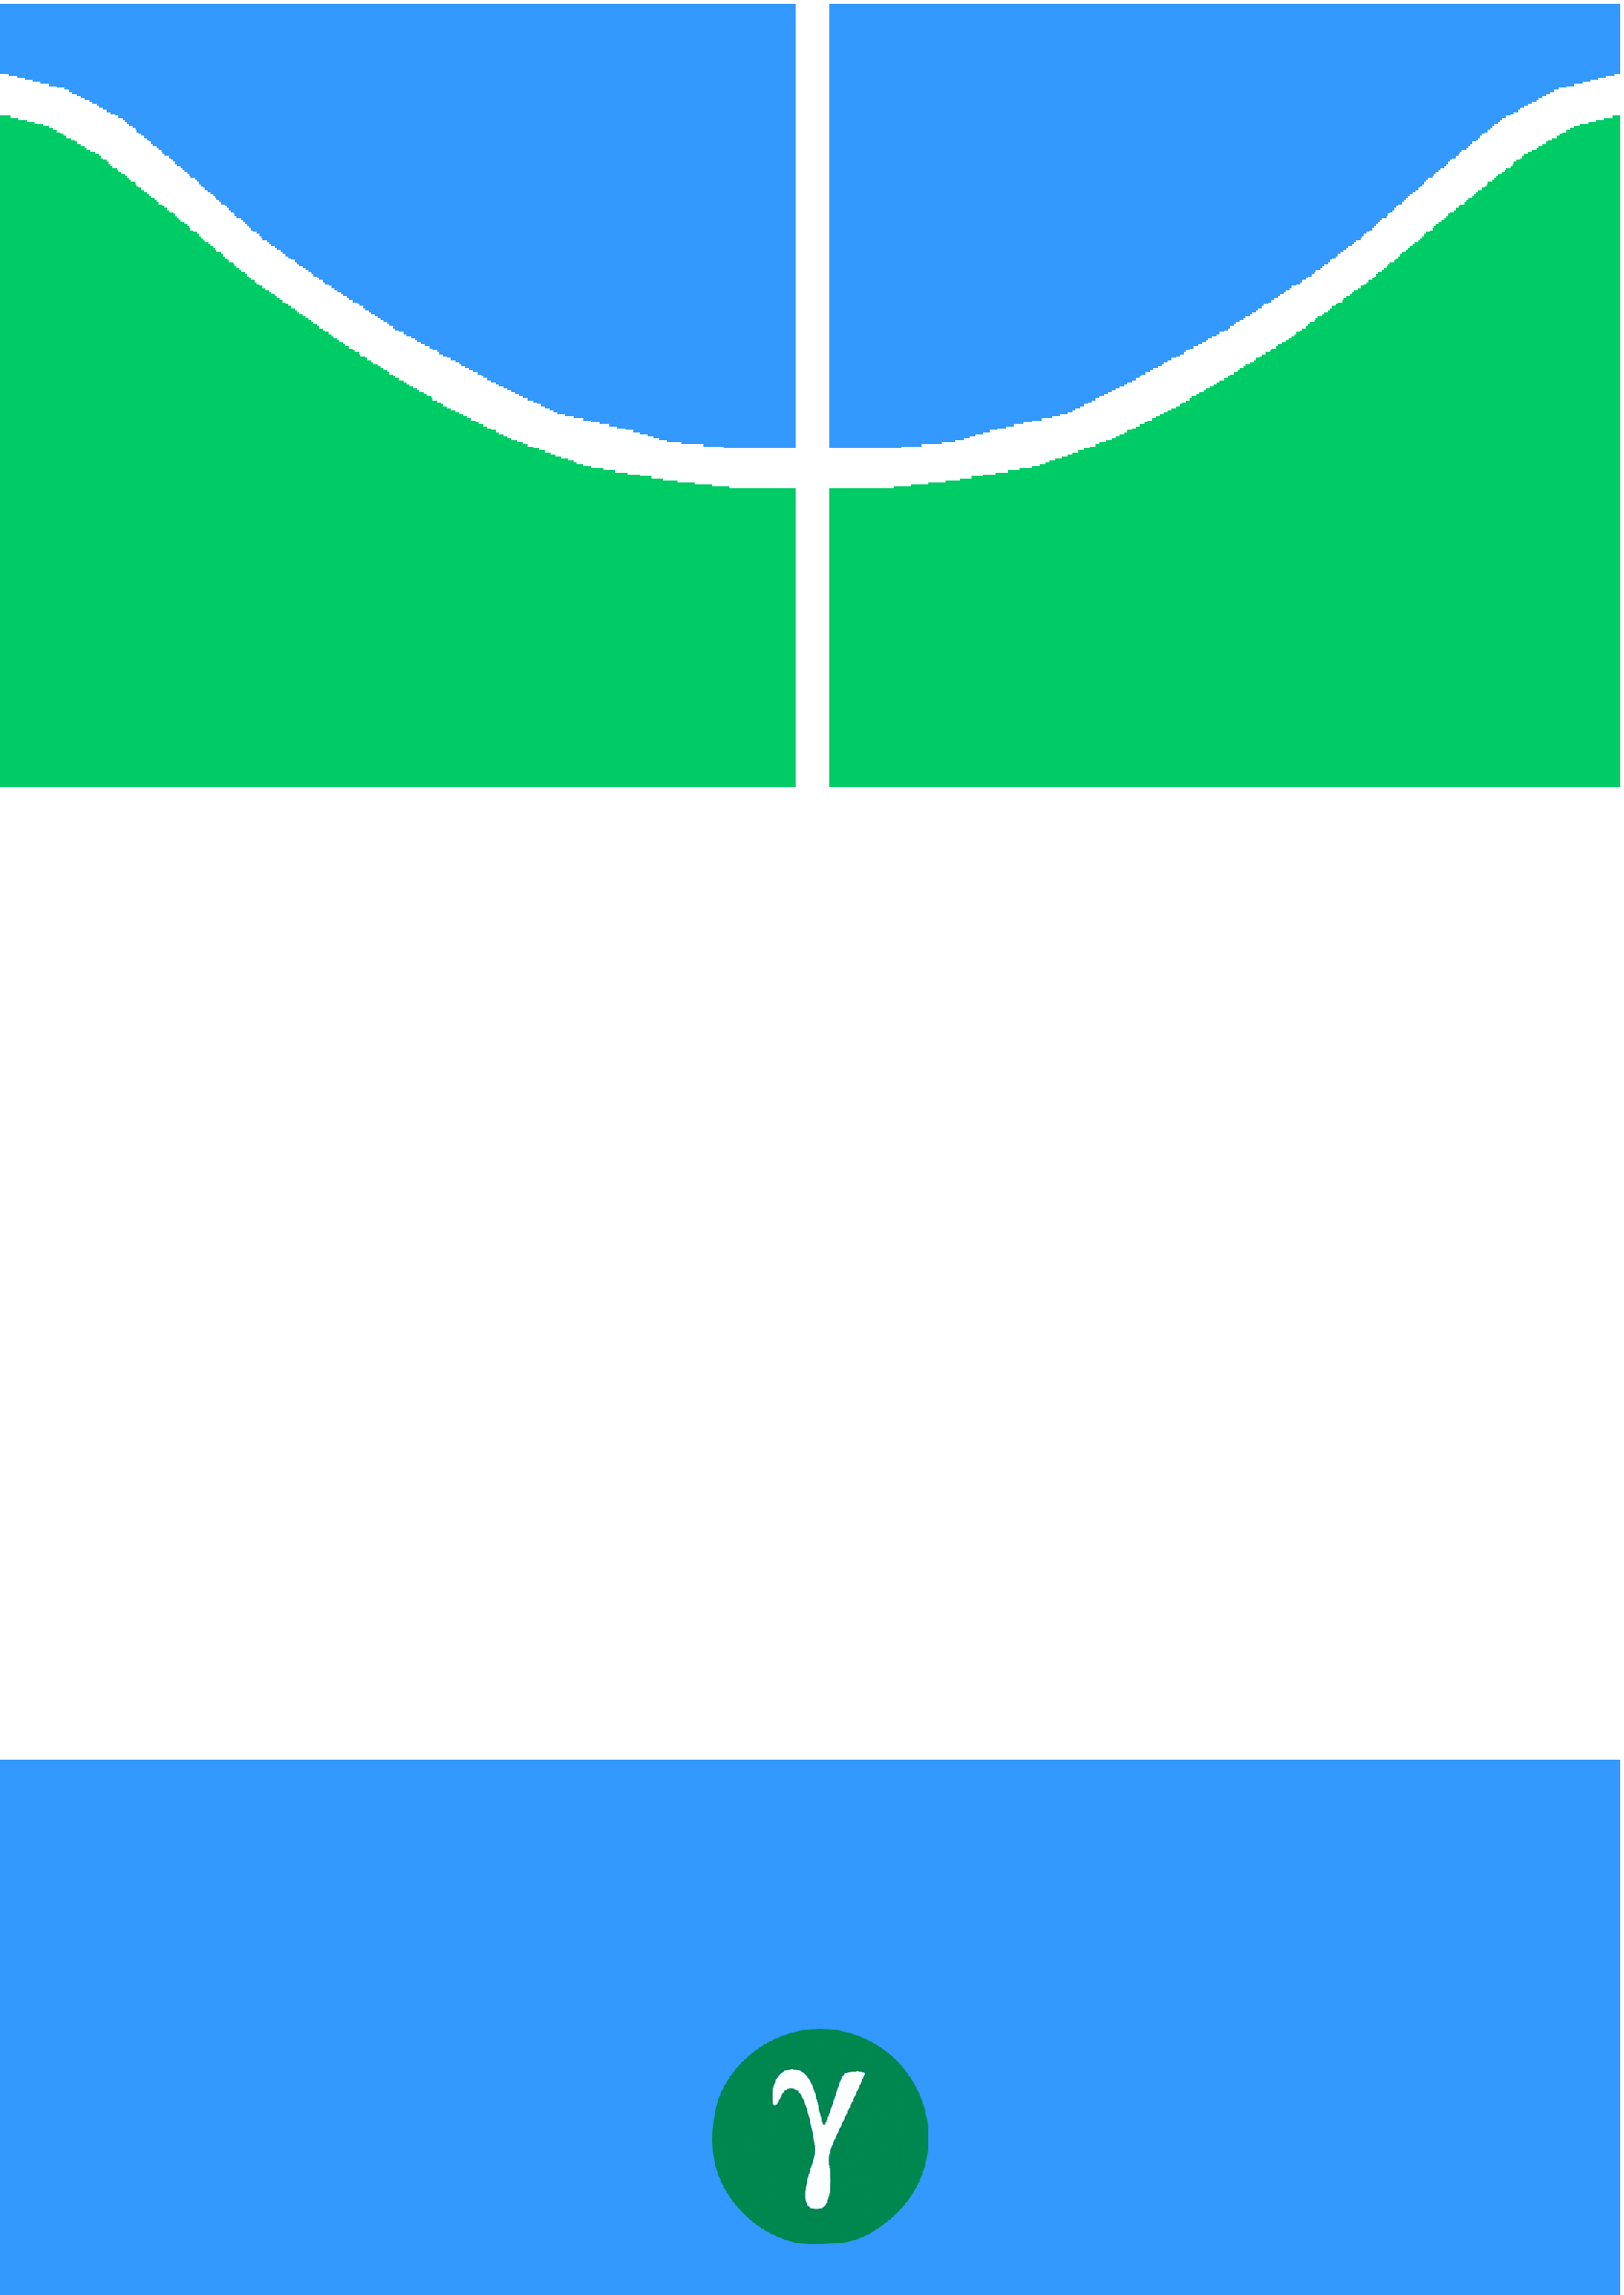
\includegraphics[width=\paperwidth,height=\paperheight,%
%				keepaspectratio]{figuras/capa.eps}%
				keepaspectratio]{figuras/capa.pdf}%
			\vfill
		}
	}
}

\renewcommand{\imprimircapa}{%
  \begin{capa}%
    \center
	\AddToShipoutPicture*{\BackgroundPic}

    \vspace*{2.7in}
	{\textbf{\large\imprimirinstituicao}}
	\par
	{\textbf{\large\imprimircurso}}

	\vspace{0.5in}

    {\ABNTEXchapterfont\bfseries\LARGE\imprimirtitulo}
    \vspace*{\fill}
    
	\begin{flushright}
    	\textbf{{\large{Autor: \imprimirautor}}}
		\par
    	\textbf{{\large{Orientador: \imprimirorientador}}}
	\end{flushright}
		
    \vspace*{0.2in}
    \textbf{{\large\imprimirlocal}}
    \par
    \textbf{{\large\imprimirdata}}
    
    \vspace*{2.2in}
  \end{capa}
}



% Dados pessoais
\autor{Brenndon Gontijo, Emilie Morais, Ítalo Paiva e Leonardo Cambraia}
\curso{Verificação e Validação}

% Dados do trabalho
\titulo{Proposta de Framework de testes para o Framework PHP CodeIgniter utilizando PHPUnit}
\data{Maio de 2016}

% Dados da orientacao
\orientador{Ricardo Ajax}

% Dados para a ficha catalográfica
\cdu{} %Não preencher

% Dados da aprovação do trabalho
\dataDaAprovacao{} %Não preencher
\membroConvidadoUm{} %Não preencher
\membroConvidadoDois{} %Não preencher

\local{Brasília, DF}
\instituicao{%
  Universidade de Brasília - UnB
  \par
  Faculdade UnB Gama - FGA
}
\tipotrabalho{Trabalho final de Verificação e Validação}
\preambulo{Trabalho final de Verificação e Validação para a disciplina de Verificação e Validação
submetido na Faculdade UnB Gama da Universidade de Brasília.}

\definecolor{blue}{RGB}{41,5,195}
\makeatletter
\hypersetup{
     	%pagebackref=true,
		pdftitle={\@title}, 
		pdfauthor={\@author},
    	pdfsubject={\imprimirpreambulo},
	    pdfcreator={LaTeX with abnTeX2},
		pdfkeywords={abnt}{latex}{abntex}{abntex2}{trabalho acadêmico}, 
		colorlinks=true,       		% false: boxed links; true: colored links
    	linkcolor=blue,          	% color of internal links
    	citecolor=blue,        		% color of links to bibliography
    	filecolor=magenta,      		% color of file links
		urlcolor=blue,
		bookmarksdepth=4
}
\makeatother
\setlength{\parindent}{1.3cm}
\setlength{\parskip}{0.2cm}  
\makeindex


\usepackage{float}
\usepackage{multirow}
\usepackage{hyperref}

\usepackage{listings}
\usepackage{color}

\definecolor{dkgreen}{rgb}{0,0.6,0}
\definecolor{gray}{rgb}{0.5,0.5,0.5}
\definecolor{mauve}{rgb}{0.58,0,0.82}

\lstset{frame=tb,
  language=Java,
  aboveskip=3mm,
  belowskip=3mm,
  showstringspaces=false,
  columns=flexible,
  basicstyle={\small\ttfamily},
  numbers=none,
  numberstyle=\tiny\color{gray},
  keywordstyle=\color{blue},
  commentstyle=\color{dkgreen},
  stringstyle=\color{mauve},
  breaklines=true,
  breakatwhitespace=true,
  tabsize=3
}

\begin{document}

\frenchspacing
\imprimircapa
% \imprimirfolhaderosto*

%% \pdfbookmark[0]{\listfigurename}{lof}
% \listoffigures*
\vfill
\pagebreak
\pdfbookmark[0]{\listtablename}{lot}
\listoftables*
\vfill
\pagebreak
\pdfbookmark[0]{\contentsname}{toc}
\tableofcontents*
\cleardoublepage


\textual

\chapter[Introdução]{Introdução}

Esse capítulo apresenta uma visão geral do trabalho através da definição do problema tratado, dos objetivos, 
da metodologia e dos resultados esperados.

\section{Problema}

Com a utilização do framework CodeIgniter, percebeu-se que o mesmo possui uma estrutura de testes muito precária, contando
apenas com uma classe de testes unitários com poucos recursos, sem a possibilidade de testes de integração. No mundo do PHP,
um dos frameworks de testes mais utilizados é o PHPUnit, que oferece diversos recursos para testes unitários e de integração.
Além disso, por ser um framework de testes bastante utilizado pela comunidade, o PHPUnit é suportado na maioria de ferramentas
de integração contínua, o que favorece ainda mais a sua utilização. Porém, o CodeIgniter não oferece suporte nativo ao PHPUnit
e existem algumas peculiaridades do CodeIgniter que devem ser levadas em conta, o que dificulta o uso do PHPUnit no CodeIgniter.

Essa deficiência em testes do framework compromete a qualidade dos sistemas que o utilizam,
como o Sistema Integrado de Gestão Acadêmica (SiGA). Portanto, a questão de pesquisa que dirige este trabalho é:

\textit{Como adequar o PHPUnit para uso no CodeIgniter?}
  
\section{Objetivos}

  Nesta seção são apresentados os objetivos geral e específicos do trabalho definidos a fim de responder a
  questão de pesquisa definida.

\subsection{Objetivo Geral}

O objetivo geral deste trabalho é elaborar um framework básico de testes para o CodeIgniter utilizando o PHPUnit, com suporte a 
testes unitários e de integração.

\subsection{Objetivos Específicos}

São objetivos específicos deste trabalho:

\begin{itemize}
 \item Adaptar o CodeIgniter para utilizar o PHPUnit;
 \item Adequar o PHPUnit para uso no CodeIgniter;
 \item Levantar features do framework de testes, com base nas necessidades do CodeIgniter;
 \item Avaliar o framework de testes criado, aplicando-o no SiGA.
\end{itemize}


\section{Metodologia}

	Como metodologia de execução do trabalho será realizada uma pesquisa-ação. De acordo com \citeonline{artigo_pesquisa_acao}, 
a pesquisa-ação pode ser caracterizada de várias formas. Para este trabalho será utilizada a pesquisa-ação iterativa e participatória.

Segundo \citeonline{artigo_pesquisa_acao}, a pesquisa-ação tem como objetivo entender uma situação em um contexto prático e melhorar esse contexto por meio de uma ação.
Dessa forma, essa metodologia foi escolhida dado o objetivo de construção de um \textit{framework} de testes para melhoria do \textit{framework} CodeIgniter.

A pesquisa-ação participatória ocorre quando o pesquisador tem uma participação ativa na implementação da ação e na produção das observações acerca do contexto estudado, também participa do compartilhamento de experiências da aplicação da ação. Uma pesquisa-ação iterativa consiste em uma ação dividida em ciclos. \cite{artigo_pesquisa_acao}

A ação a ser proposta é composta de um diagnóstico que é definido por \citeonline{artigo_pesquisa_acao} como uma fase que tem como objetivo principal conhecer a situação atual. Os ciclos de ação definidos para este trabalho tem como base as outras fases definidas por \citeonline{artigo_pesquisa_acao}: Planejamento da ação, Execução da ação e Avaliação da ação.

No diagnóstico serão estudados:
	\begin{itemize}
		\item O \textit{framework} de testes PHPUnit para entender as suas funcionalidades;
		\item O \textit{framework} CodeIgniter para entender como adequá-lo para uso do PHPUnit;
		\item Serão definidas todas as \textit{features} do \textit{framework} a ser criado.
	\end{itemize}

Para cada ciclo serão planejadas as atividades a serem realizadas para implementação do \textit{framework}.
Após o planejamento, essas atividades serão realizadas.
No final de cada ciclo será realizada uma avaliação do \textit{framework} por meio
de sua aplicação em um sistema (Sistema Integrado de Gestão Acadêmica - SiGA). A partir dessa aplicação serão identificadas
melhorias para as \textit{features} implementadas e até possíveis novas \textit{features}. 

A avaliação do \textit{framework} proposto e a identificação de melhorias serão realizadas por meio da avaliação qualitativa 
das respostas ao questionário (Apêndice \ref{questionario}) que será aplicado a dois desenvolvedores do sistema SiGA após utilizarem
o \textit{framework} para realizar determinados testes.


\section{Resultados Esperados}

Como resultado é esperado um \textit{framework} básico de testes para ser utilizado no \textit{framework} CodeIgniter, que contemple
testes unitários e testes de integração. Com a utilização da pesquisa-ação também é esperado que o \textit{framework} seja realmente adequado
ao CodeIgniter. 

\section{Cronograma}

A execução do trabalho foi organizada conforme Figura \ref{fig:cronograma}.

\begin{figure}[!htb]
% \centering
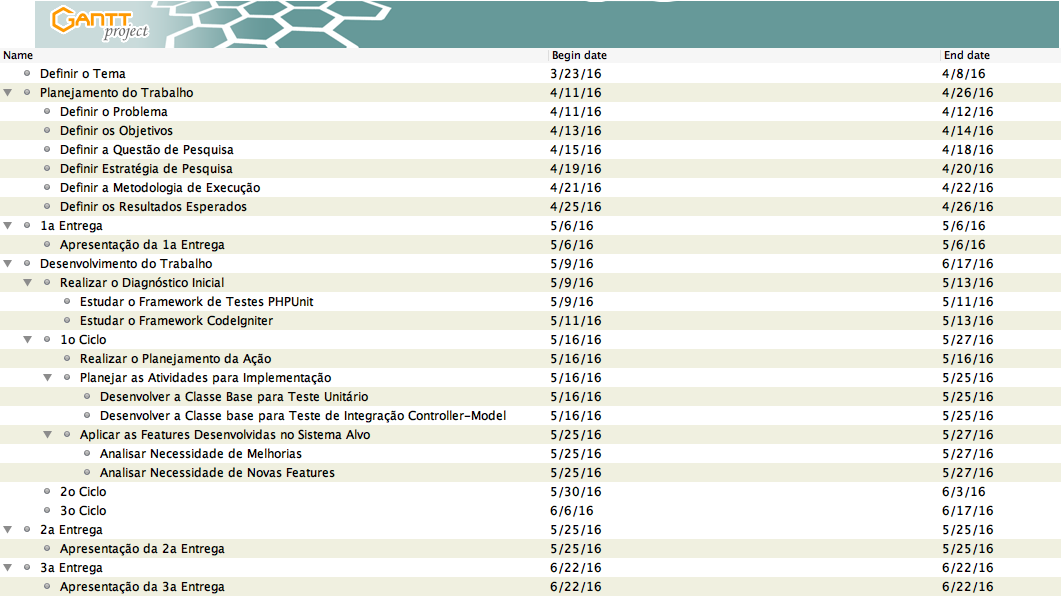
\includegraphics[scale=0.45]{figuras/Cronograma.png}
\caption{Cronograma}
\label{fig:cronograma}
\end{figure}

\chapter{Referencial Teórico}
Para realizar o levantamento do referencial teórico foi utilizado a técnica de revisão de literatura.
Segundo \citeonline{revisao_de_literatura}, uma revisão de literatura comporta uma parte muito importante no processo de investigação, 
uma vez estabelecida por localizar, analisar, sintetizar e interpretar a investigação prévia referente a uma área de estudo. 
Além disso, uma boa revisão de literatura auxilia no entendimento de um problema e desenvolvimento dos conhecimentos, 
conforme \apudonline{livro_sistematizacao_conhecimento}{revisao_de_literatura}, “cada investigador analisa minuciosamente os trabalhos dos investigadores 
que o precederam e, só então, compreendido o testemunho que lhe foi confiado, parte equipado para a sua própria aventura”, 
ou seja, ao se iniciar o processo de revisão de literatura raramente não existirão assuntos abordados no passado, sobre o 
mesmo tema ou similares, que auxiliarão como fonte de conhecimento para a atual pesquisa.

Novamente, segundo \citeonline{revisao_de_literatura}, os propósitos da revisão de literatura num estudo de investigação são:

\begin{itemize}
 
	\item \textbf{Delimitar o problema de investigação:} formular uma definição concreta sobre o que será investigado visando não comprometer todo o trabalho com problemas mal delimitados.
	\item \textbf{Procurar novas linhas de investigação:} consiste em entender o que já foi realizado sobre um determinado problema e buscar pelas suas áreas que ainda não foram ou foram pouco exploradas.
	\item \textbf{Evitar abordagens infrutíferas:} buscar que as linhas de investigação definidas sejam proveitosas e possuam resultados significativos.
	\item \textbf{Ganhar perspectivas metodológicas:} não rever apenas os resultados do estudo, mas sim, realizar uma leitura geral sobre todos os tópicos abordados.
	\item \textbf{Identificar recomendações para investigações futuras:} após finalizado o estudo, identificar novas questões e sugestões para investigações futuras.

\end{itemize}

O referencial teórico deste trabalho contemplará os conceitos de:

\begin{itemize}

	\item Testes unitarios
	\item Testes de integração
	\item \textit{Framework} de testes
	
\end{itemize}


\chapter{Diagnóstico}

Neste capítulo são apresentados os resultados do diagnóstico realizado.

\section{\textit{Features} do \textit{framework}}

\begin{itemize}

	\item Classe base para teste unitário
	\item Classe base para teste de integração controller-model
	\item Elaborar esquema de criação de dados no banco de dados (\textit{migration} de teste)
	\item Reconhecimento da \textit{controller} que está sendo testada
		\subitem Ex: CourseTest (Classe de Teste) -> Course (\textit{Controller})
	\item Fazer esquema de subir o banco pro teste e depois limpar o banco
	\item Elaborar uma forma para criar dados fixos para o banco de teste (similar ao Bootstrap do Grails);
	\item Classe base para teste de helper
	\item Classe base para teste de módulo
	\item Classe base de teste funcional
	\item Fazer \textit{mock}

\end{itemize}
\chapter{Ciclo 1}
  
  Este capítulo descreve o planejamento realizado e os resultados obtidos com a execução do primeiro ciclo da pesquisa-ação.
  
  \section{Planejamento}
  
      Após a realização do diagnóstico, era necessário um esforço inicial de configuração do \textit{framework} para a 
      adequação do PHPUnit ao CodeIgniter. Além disso, era necessário estabelecer a estrutura do \textit{framework},
      sua arquitetura de funcionamento. Portanto, ficaram definidas como escopo do primeiro ciclo as seguintes atividades:
      
      \begin{itemize}
    
    \item Configurar o CodeIgniter para receber o PHPUnit;
    
    \item Estabelecer arquitetura de funcionamento do \textit{framework}.
    
      \end{itemize}
      
      
      \subsection{Planejamento da avaliação}
      
      Como este ciclo não agregou muito valor para a atividade de testes dos desenvolvedores do SiGA,
      embora imprescindível para o \textit{framework}, o mesmo teve uma forma de avaliação diferente
      dos outros ciclos (não avaliado pelo questionário proposto) por não envolver diretamente os desenvolvedores e se
      tratar de conteúdo mais técnico inerente à equipe de desenvolvimento do \textit{framework}. Visto isso, ficou proposta
      a seguinte estrutura de avaliação para as atividades realizadas neste ciclo:
      
      \begin{itemize}
      
        \item Para a atividade de configuração do CodeIgniter para o uso do PHPUnit:
      
        \begin{enumerate}
          
          \item Testar as configurações propostas em um projeto vazio do CodeIgniter versão 2.x;
          
          \item Testar as configurações propostas no SiGA;
          
        \end{enumerate}
          
        \item Para a atividade de estabelecimento da arquitetura de funcionamento do \textit{framework}:
        
        \begin{enumerate}
    
          \item Validar a arquitetura proposta implementando os comandos \textit{\textbf{init}} e \textit{\textbf{help}};
              
              \subitem Se atentar aos seguintes itens indispensáveis:
            \begin{itemize}
              \item É fácil de se criar um novo comando?
              \item É possível criar um comando com parâmetros diferentes?
              \item É possível ter parâmetros opcionais nos comandos?
              \item É possível tratar cada comando individualmente e executá-los em conjunto?
            \end{itemize}
          
          \item Testar o comando \textit{\textbf{init}} em um projeto vazio do CodeIgniter versão 2.x;
          
          \item Testar o comando \textit{\textbf{init}} no SiGA;
    
          \item Testar o comando \textit{\textbf{help}};
        \end{enumerate}
      
      \end{itemize}
  
  \section{Execução do ciclo}
  
      Esta seção apresenta detalhes relacionados à execução do ciclo 1.
      
      \subsection{Arquitetura do \textit{Ignitest}}
      
	  Para o contexto proposto, onde existirão vários comandos que possuem comportamentos únicos e bem definidos que serão
	  invocados pela linha de comando, a arquitetura definida se baseia no padrão de projeto \textit{Command} \cite{gamma}
	  com a adição de classes \textit{experts} (padrão GRASP) de metadados para cada comando, como pode ser visto na
	  figura \ref{ignitest-architecture}.
	   
	  As classes filhas da classe \textit{Command} representam um comando específico do \textit{framework} que possui sua 
	  própria implementação de execução. Cada comando possui uma classe de metadados associada a ele para descrever suas
	  informações, onde essa classe deve herdar da classe \textit{Metadata}. Os comandos informados pela linha de comando (CLI)
	  são interpretados pela classe \textit{CommandChecker}, que verifica os comandos informados, cria as instâncias respectivas
	  e adiciona os comandos na fila de execução. Os comandos disponíveis no \textit{framework} devem ser registrados na classe
	  \textit{AvailableCommand} para que seja possível a classe \textit{CommandChecker} identificar os comandos informados.
	  
	  \vfill
	  \pagebreak
	  \begin{figure}[!htb]
	    \centering
	    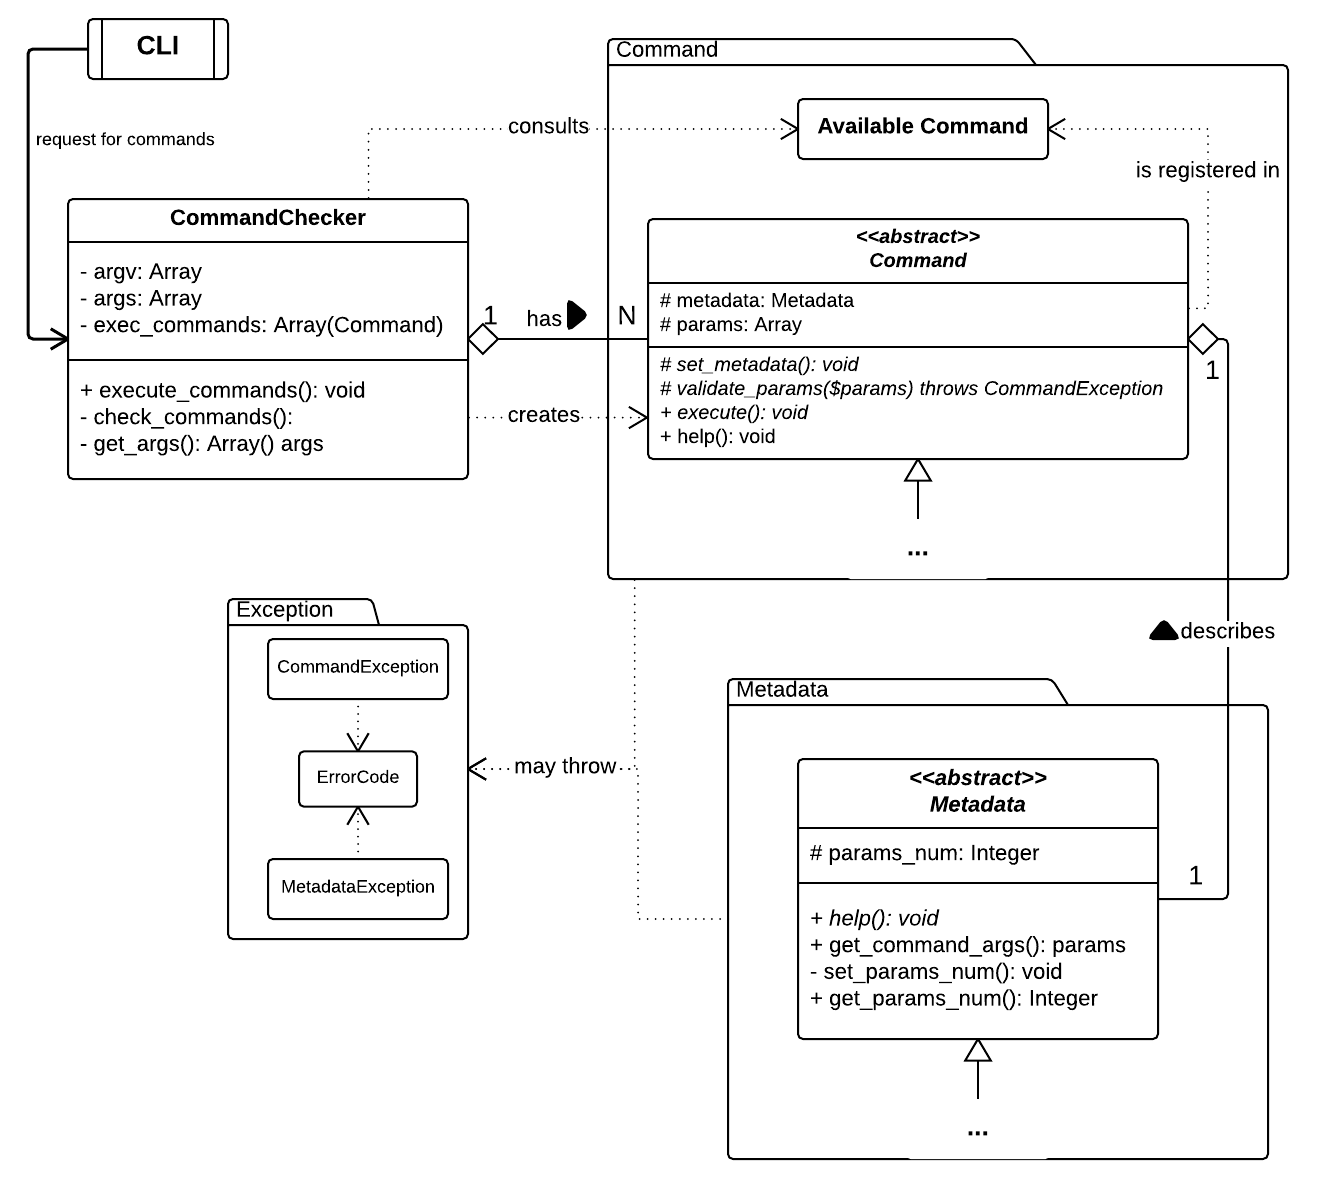
\includegraphics[scale=0.35]{figuras/ignitest-architecture.png}
	    \caption{Arquitetura do \textit{framework} proposto.}
	    \label{ignitest-architecture}
	  \end{figure}
      
      \subsection{Configurações}
	  
	  Para que o PHPUnit funcione no CodeIgniter, descobriu-se que era preciso definir um \textit{hook}\footnotemark
	  no projeto para mostrar os resultados do PHPUnit caso o ambiente fosse de teste, pois ao executar o PHPUnit nenhum
	  resultado era disponibizado na tela. Foi preciso seguir os seguintes passos para resolver esse problema:
	  \footnotetext{CodeIgniter Hooks. Disponível em \url{http://www.codeigniter.com/userguide2/general/hooks.html}. Acesso em 20/06/2016.}
	  
	  \begin{itemize}
	  
	   \item Habilitar o uso de \textit{hooks} no CodeIgniter no arquivo '\textbf{application/config/config.php}':
	      
	      \begin{verbatim}
		$config['enable_hooks'] = TRUE;
	      \end{verbatim}
	      
	   \vfill
	   \pagebreak
	   \item Criar o seguinte \textit{array} no arquivo '\textbf{application/config/hooks.php}':
	  
	      \begin{lstlisting}
		$hook['display_override'] = array(
		    'class' => 'DisplayHook',
		    'function' => 'captureOutput',
		    'filename' => 'DisplayHook.php',
		    'filepath' => 'hooks'
		);
	      \end{lstlisting}
	   
	   \item Criar a seguinte classe no diretório '\textbf{/application/hooks/}' sob o nome '\textbf{DisplayHook.php}':
	  
	  \begin{lstlisting}
	  
	      <?php
	      
	      class DisplayHook {
	          public function captureOutput() {

	              $this->CI =& get_instance();
			  
	              $output = $this->CI->output->get_output();

	              if (ENVIRONMENT != 'testing') {
	                  echo $output;
	              }
	          }
	      }
	  \end{lstlisting}
	  
	  \end{itemize}
	  
	  Além dos passos acima, são necessárias as configurações essenciais do PHPUnit, que são descritas abaixo:
	  
	  \begin{itemize}
	    \item Criar o arquivo de configuração do PHPUnit '\textbf{\textit{phpunit.xml}}' 
		  no diretório '\textbf{application/tests/}';
	    
	    \item Criar o arquivo de inicialização para os testes '\textbf{\textit{bootstrap.php}}'
		  no diretório '\textbf{application/tests/}';
	      
		\subitem Este arquivo é executado antes dos testes. Para o uso no CodeIgniter, esse arquivo deve ser
			 adaptado para conter o mesmo conteúdo do arquivo de inicialização do CodeIgniter '\textbf{index.php}', 
			 para que os recursos do CodeIgniter estejam disponíveis durante os testes.
	  \end{itemize}
	  
	  Durante a execução do ciclo, percebeu-se que era necessária bastante configuração para que o PHPUnit rodasse no
	  CodeIgniter e, portanto, parte dessa configuração, as configurações essenciais do PHPUnit, foi abstraída para
	  dentro do \textit{framework} no comando \textit{\textbf{init}}, para diminuir a carga de configuração
	  para o desenvolvedor.
 
  \section{Resultados obtidos}
    
      Este ciclo produziu os seguintes resultados:
      
      \begin{itemize}

    \item Configuração do PHPUnit ao CodeIgniter estabelecida;
    
    \item Arquitetura do \textit{framework} estabelecida;
    
    \item Comando \textit{\textbf{init}}, para automatizar parte da configuração.

      \end{itemize}

  \section{Avaliação dos resultados}
      Esta seção descreve os resultados das avaliações de configurações e arquitetura propostas, bem como pontos a serem melhorados.

      \subsection{Avaliação das configurações}
      
	  Ao tentar aplicar as configurações propostas em um novo projeto do CodeIgniter, ocorreram alguns erros referentes
	  à configuração do PHPUnit com o CodeIgniter, as quais foram sanadas da seguinte forma:
	  
	  \begin{itemize}

	    \item Configuração de protocolo URI: o protocolo em questão não pode ser automático, assim, foi necessário modificá-lo para
	    o tipo "REQUEST\_URI".
	    
	    \item Classe CI\_Utf8: era necessário carregar as configurações do CodeIgniter ao inicializar a classe.

	  \end{itemize}
	  
	  No sistema SiGA foram identificados os mesmos erros referentes às configurações.
      
      \subsection{Avaliação da arquitetura}
	  Percebeu-se que a arquitetura do \textit{framework} foi bem estrutura com o uso do padrão de projeto \textit{Command}, 
	  uma vez que facilmente é possivel criar novos comandos definindo-se uma classe para o mesmo e adicionando-o aos comandos
	  existentes.
	  
	  A criação de um comando com parâmetros diferentes foi identificada e possível graças aos metadados vinculados ao mesmo, 
	  os quais podem descrever a quantidade de parâmetros que um comando possuirá, além disso, cada metadado define como os 
	  argumentos do comando serão coletados, ou seja, caso hajam argumentos opcionais basta que os mesmos sejam tratados.
	  
	  Foi possível realizar a execução de vários comandos em conjunto, uma vez que o módulo \textit{CommandChecker} se encarrega 
	  de identificar os comandos enviados, validá-los e adicioná-los à fila de execução.
	  
	  Não ocorreram problemas ao executar os comandos \textit{init} e \textit{help} em um projeto vazio e no SiGA. 
	  
      
      \subsection{Melhorias identificadas}
	  Com todas as dificuldades encontradas durante a avaliação, percebeu-se que seria interessante embutir no comando 
	  \textit{\textbf{init}} todas as configurações realizadas manualmente, para que novos usuários não tenham tais problemas.
    

\chapter{Ciclo 2}

  Este capítulo descreve o planejamento realizado e os resultados obtidos com a execução do segundo ciclo da pesquisa-ação.
  
  \section{Planejamento}
  
    Para compor o escopo do segundo ciclo ficaram alocadas as seguintes funcionalidades, com suas respectivas características:
    
      
    \begin{itemize}
      
        \item \textbf{Criação da classe base para testes unitários;}
    
            \begin{itemize}
              \item Reconhecimento da classe que está sendo testada por convenção de nomenclatura;

            \end{itemize}
     
        \item \textbf{Classe base para testes de integração.}
    
            \begin{itemize}
              \item Reconhecimento da classe que está sendo testada por convenção de nomenclatura;
              \item Esquema de criação e destruição do banco de testes;
              \item Definição de dados iniciais no banco de testes;
            
            \end{itemize}
    
        \item Criação do comando \textit{\textbf{create\_unit}}, para automatizar a criação da classe de teste para teste unitário de \textit{domains}.
        
        \item Criação do comando \textit{\textbf{create\_integration}}, para automatizar a criação da classe de teste para teste de integração de \textit{controllers}.
    
    \end{itemize}

  \section{Execução do ciclo}
      
    \subsection{Classe base para testes unitários}

        Foi implementada uma classe base, chamada \textbf{UnitCaseTest}, que deve ser herdada de todas as classes de teste de integração criadas. 
        Essa classe base herda da classe \textbf{PHPUnit\_Framework\_TestCase}. Sendo assim as classes de teste unitário criadas através do \textit{framework} herdam as funcionalidades do PHPUnit e a funcionalidade proposta para a classe base.

        Para a classe base a proposta é reconhecer a classe de domínio que será testada, verificando sua existência e já disponibilizando-a para uso (importando) na classe de testes. No código apresentado abaixo, o método \textit{class\_under\_test} é responsável por identificar a classe a ser testada e importá-la. No método \textit{search\_class\_file} é verificada a existência da classe que o desenvolvedor deseja testar. O método \textit{setUp} será executado antes da execução de cada teste e pode ser sobreescrito nas classes de teste criadas, contanto que também execute o método da classe base.  

        \begin{lstlisting}
            <?php

            require_once APPPATH.'/tests/ignitest/src/exception/TestException.php';

            abstract class UnitCaseTest extends PHPUnit_Framework_TestCase{

                protected $ci;
                protected $testClass;

                private function class_under_test($child){
                    $className = get_class($child);

                    $name = str_replace("Test", "", $className);
                    $capitalizeName = ucfirst($name);

                    $file_path = $this->search_class_file($capitalizeName);

                    if (!empty($file_path)) {
                        require_once $file_path;
                    }
                    else{
                        throw new TestException("File could not be found", 0);
                    }
                }

                public function search_class_file($class_name){
                    $file_path = "";

                    $it = new RecursiveDirectoryIterator(DOMAINPATH);
                    foreach (new RecursiveIteratorIterator($it) as $file) {
                        $file_name = $file->getFileName();
                        if($file_name == $class_name.".php"){
                            $file_path = $file->getPathName();
                            break; 
                        }
                    }

                    return $file_path;
                }
                
                public function setUp() {   

                    $this->classUnderTest($this);
                    $this->ci =& get_instance();
                }
            }

        \end{lstlisting}

    \subsection{Classe base para testes de integração}

        Para o \textit{Ignitest} foi criada uma classe base chamada \textbf{IntegrationTestCase} que deve ser herdada de todas as classes de teste unitário criadas. 
        Essa classe base herda da classe \textbf{PHPUnit\_Extensions\_Database\_TestCase}. Sendo assim as classes de teste de integração criadas através do \textit{framework} herdam as funcionalidades do PHPUnit e a funcionalidade proposta para a classe base.

        Para a classe base a proposta é reconhecer a \textit{controller} que será testada, verificando sua existência e já disponibilizando-a para uso (importando) na classe de testes. No código apresentado abaixo, o método \textit{class\_under\_test} é responsável por identificar a classe a ser testada e importá-la. No método \textit{search\_class\_file} é verificada a existência da classe que o desenvolvedor deseja testar. O método \textit{setUp} será executado antes da execução de cada teste e pode ser sobreescrito nas classes de teste criadas, contanto que também execute o método da classe base. Além de importar a classe que está sendo testada, a classe do \textit{Ignitest} também já cria e disponibiliza a instância da classe.

        \begin{lstlisting}
            <?php

            include "config_ignitest.php";

            abstract class IntegrationTestCase extends PHPUnit_Extensions_Database_TestCase{

              static private $pdo = null;
              private $conn = null;

              protected $ci;
                protected $testClass;

                /**
                 * @Override
                 */
              final public function getConnection(){
                if ($this->conn === null) {
                  if (self::$pdo == null) {
                    $pdo_data = "mysql:dbname=".DATABASE_NAME.";host=".HOST;
                    self::$pdo = new PDO($pdo_data, USERNAME, PASSWORD);
                  }

                  $this->conn = $this->createDefaultDBConnection(self::$pdo, DATABASE_NAME);
                }
                return $this->conn;
              }

              /**
                 * @Override
                 */
              public function getDataSet(){
                return $this->createMySQLXMLDataSet(DATASET);
              }

              private function classUnderTest($child){
                    $className = get_class($child);

                    $name = str_replace("Test", "", $className);

                    $file_path = $this->search_class_file($name);

                    if (!empty($file_path)) {
                        require_once $file_path;

                        $name = ucfirst($name);
                        $this->testClass = new $name();
                    }
                    else{
                        throw new TestException("File could not be found", 0);
                    }
                }

                private function search_class_file($class_name){
                    $file_path = "";

                    $it = new RecursiveDirectoryIterator(CONTROLLERPATH);
                    foreach (new RecursiveIteratorIterator($it) as $file) {
                        $file_name = $file->getFileName();
                        if($file_name == strtolower($class_name).".php" || $file_name == ucfirst($class_name).".php"){
                            $file_path = $file->getPathName();
                            break; 
                        }
                    }

                    return $file_path;
                }

              public function setUp(){
                parent::setUp();
                $this->classUnderTest($this);
                    $this->ci =& get_instance();
              }
            }
    \end{lstlisting}

%       % Sincronização dos banco de dados.

    \subsection{Criação dos comandos}

        Foram criados dois comandos para criação das classes de teste, um para criar a classe de teste unitário e outra para a de integração, seguindo a arquitetura 
        proposta no ciclo 1, através do padrão de projeto \textit{Command}. 

        O comando \textit{create\_unit <class name>} cria uma classe de teste unitário para a classe passada como argumento no comando, caso esta classe de domínio exista. Esta classe de teste herda da classe base \textbf{UnitCaseTest} e dessa forma importa a classe de domínio que está sendo testada.

        O comando \textit{create\_integration <class sname>} cria uma classe de teste de integração para a classe passada como argumento no comando, caso esta classe \textit{controller} exista. Esta classe de teste herda da classe base \textbf{IntegrationTestCase} e dessa forma importa a \textit{controller} que está sendo testada e cria uma instância desta.

        Quando a classe passada como argumento para ambos os comandos já possui uma classe de teste associada, para criar novamente e substituir o código escrito foi acrescentado ao comando o argumento opcional \textit{-force} ou \textit{-f}. 

  
  \section{Resultados obtidos}
      
    \begin{itemize}

      \item Classe base de teste unitário criada, com reconhecimento da classe de domínio a ser testada;
      
      \item Classe base de teste de integração criada, com reconhecimento e instância da \textit{controller} que está sendo testada;
            
      \item Comando \textit{\textbf{create\_unit}}, para criar classe de teste unitário;

      \item Comando \textit{\textbf{create\_integration}}, para criar classe de teste de integração.

    \end{itemize}
  
  \section{Avaliação dos resultados}

    Para avaliar os resultados deste ciclo dois desenvolvedores do SiGA realizaram testes para uma classe utilizando o método padrão de implementação do CodeIgniter e o \textit{framework}. Após a implementação os desenvolvedores responderam a um questionário, que pode ser visto no Apêndice \ref{questionario}. 

    Considerando as respostas dos desenvolvedores foi possível perceber que
  
    \subsection{Melhorias identificadas}
    
\chapter{Ciclo 3...n}
  
  O tempo para a realização do trabalho não permitiu a execução de mais de um
  ciclo,embora o planjemento inicial tenha previsto mais de um ciclo. Todavia, sabe-se que o escopo dos próximos
  ciclos seria estabilizar as funcionalidades propostas do \textit{framework} com base nas melhorias identificadas
  no final de cada ciclo.
  
  A quantidade de ciclos foi estabelecida como indefinida, pois seriam executados
  ciclos até que o \textit{framework} se tornasse estável.
  
\chapter{Conclusão}




\bookmarksetup{startatroot}

\postextual


\bibliography{bibliografia}{}
\begin{apendicesenv}

\partapendices

\chapter{Questionário de Avaliação do Framework}
\label{questionario}

    Para assegurar a viabilidade do uso do \textit{Ignitest} (\textit{framework} proposto), foi elaborado pelos autores, um questionário a ser respondido pelos testadores responsáveis pela avaliação.
    
    As perguntas a seguir estão divididas nas categorias: Documentação, Resultados (propõe comparações entre a criação de testes usando apenas a classe de testes padrão do \textit{CodeIgniter}, aqui chamado de método padrão, e o \textit{Ignitest}) e \textit{Feedback}.
    
    \begin{itemize}
        \item Documentação
        
            Com base na documentação presente no repositório do \textit{Ignitest}\footnote{https://github.com/VerVal-2016-1/Framework}, responda:
            \begin{itemize}
                \item Com as informações presentes na seção "Instalação", foi possível instalar o \textit{Ignitest} sem dificuldades?
                \item Com as informações presentes na seção "Instruções", foi possível entender o funcionamento do \textit{Ignitest}?
            \end{itemize}
            
        \item Resultados
            \begin{itemize}
                \item Tempo
                    \begin{enumerate}
                        \item Qual o tempo gasto para testar uma determinada classe, usando o método padrão?
                        \item Qual o tempo gasto para testar a mesma classe com o auxílio do \textit{Ignitest}?
                    \end{enumerate}
                \item Dificuldades
                    \begin{enumerate}
                        \item Existem dificuldades em testar usando o método padrão? Se sim, quais?
                        \item Essas dificuldades foram reduzidas, ou sanadas, com o uso do \textit{Ignitest}?
                        \item Novas dificuldades apareceram com o uso do \textit{Ignitest}? Se sim, quais?
                    \end{enumerate}
                \item Quantidade de código
                    \begin{enumerate}
                        \item Usando o método padrão, quantas linhas de código foram escritas para o teste da classe escolhida?
                        \item Com o uso do \textit{Ignitest}, quantas linhas de código foram escritas para o teste da mesma classe?
                    \end{enumerate}

\vfill
\pagebreak

                \item Erros
                    \begin{enumerate}
                        \item Usando o método padrão, quantos erros ao inserir comandos você cometeu?
                        \item Com o \textit{Ignitest}, quantos erros ao inserir comandos você cometeu?
                    \end{enumerate}
            \end{itemize}
        
        \item \textit{Feedback}
            \begin{itemize}
                \item Como foi sua experiência usando o \textit{Ignitest}?
                \item Durante o uso do \textit{Ignitest}, recebeu alguma mensagem de erro?
                \item Durante o uso, o \textit{Ignitest} deixou de funcionar em algum momento?
                \item Possui alguma sugestão de melhoria?
            \end{itemize}
    \end{itemize}

    %%% tempo de teste 2 atributos italo 45 min
    %%% 3 erros

\chapter{Respostas da entrevista - Desenvolvedor 1}
    
    \begin{itemize}
        \item Documentação
        
            Com base na documentação presente no repositório do \textit{Ignitest}\footnote{https://github.com/VerVal-2016-1/Framework}, responda:
            \begin{itemize}
                \item \textbf{Com as informações presentes na seção "Instalação", foi possível instalar o \textit{Ignitest} sem dificuldades?}
		    
		    \subitem \textit{O processo de instalação do Framework é bastante simples e, embora simples, está bem documentado no 
			      repositório do Framework}.
		    
                \item \textbf{Com as informações presentes na seção "Instruções", foi possível entender o funcionamento do \textit{Ignitest}?}
		     
		     \subitem \textit{As funcionalidades do Framework estão bem descritas no repositório, com suas respectivas configurações.
			      Foi bastante simples entender como usar o Framework}.
		     
            \end{itemize}
            
        \item Resultados
            \begin{itemize}
                \item Tempo
                    \begin{enumerate}
                        \item \textbf{Qual o tempo gasto para testar uma determinada classe, usando o método padrão?}
			  
			  \subitem \textit{Foram gastos 45 minutos utilizando o método padrão para realizar a implementação de 15 casos de testes.}
			  
                        \item \textbf{Qual o tempo gasto para testar a mesma classe com o auxílio do \textit{Ignitest}?}
			  
			  \subitem \textit{Para os mesmos 15 casos de testes, foram gastos 16 minutos utilizando o Ignitest.}
                        
                    \end{enumerate}
                \item Dificuldades
                    \begin{enumerate}
                        \item \textbf{Existem dificuldades em testar usando o método padrão? Se sim, quais?}
                        
			  \subitem \textit{Sim. No método padrão é necessário criar uma controller para representar a classe de teste,
				    criar uma rota para a controller de teste para poder visualizar os resultados dos testes, para ai
				    poder começar os testes. Com um teste criado, é necessário chamá-lo no método index para aparecer
				    o seu resultado relatório, ou seja, todos os testes criados devem ser chamados no método index para
				    conseguir ver algum resultado}.
			  
                        \item \textbf{Essas dificuldades foram reduzidas, ou sanadas, com o uso do \textit{Ignitest}?}
                        
			  \subitem \textit{Com o Ignitest não é preciso mais criar controllers de testes e nem as rotas. Basta criar 
				    a classe de teste e começar os testes. Para ver os resultados do testes também é muito simples, 
				    se resume a um comando!}.
			  
                        \item \textbf{Novas dificuldades apareceram com o uso do \textit{Ignitest}? Se sim, quais?}
                        
			  \subitem \textit{Até então, não}.
			  
                    \end{enumerate}
                \item Quantidade de código
                    \begin{enumerate}
                        \item \textbf{Usando o método padrão, quantas linhas de código foram escritas para o teste da classe escolhida?}
			  
			  \subitem \textit{Com o método padrão o código dos testes possuem em média 8-12 linhas, são muito extensos.
				    Para os 15 casos de testes implementados, foram necessárias 350 linhas em média}.
			  
                        \item \textbf{Com o uso do \textit{Ignitest}, quantas linhas de código foram escritas para o teste da mesma classe?}
			  
			  \subitem \textit{Com o Ignitest o código dos testes se resumiram a 5 linhas em média, o que deixou a classe
				    de testes bastante enxuta, com 175 linhas em média}.
			  
                    \end{enumerate}

                \item Erros
                    \begin{enumerate}
                        \item \textbf{Usando o método padrão, quantos erros ao inserir comandos você cometeu?}
                        
			  \subitem \textit{Foram cometidos 3 erros em relação a adição de dependências na classe de testes e
				    com a definição das rotas.}.
			  
                        \item \textbf{Com o \textit{Ignitest}, quantos erros ao inserir comandos você cometeu?}
			  
			  \subitem \textit{Nenhum erro crítico, apenas erros de digitação do comando}.
                    \end{enumerate}
            \end{itemize}
        
        \item \textit{Feedback}
            \begin{itemize}
                \item \textbf{Como foi sua experiência usando o \textit{Ignitest}?}
		    
		   \subitem \textit{A experiência foi boa. Foi gasto menos tempo com os testes e código do teste está mais
			    enxuto, limpo e elegante}.
		  
                \item \textbf{Durante o uso do \textit{Ignitest}, recebeu alguma mensagem de erro?}
                
		   \subitem \textit{Não}.
		   
                \item \textbf{Durante o uso, o \textit{Ignitest} deixou de funcionar em algum momento?}
                
		   \subitem \textit{Não}.
		   
                \item \textbf{Possui alguma sugestão de melhoria?}
                
		   \subitem \textit{Criar um executável para o Framework, para facilitar a instalação e o uso}.
            \end{itemize}
    \end{itemize}
\chapter{Respostas da Entrevista - Desenvolvedor 2}
    
    \begin{itemize}
        \item Documentação
        
            Com base na documentação presente no repositório do \textit{Ignitest}\footnote{https://github.com/VerVal-2016-1/Framework}, responda:
            \begin{itemize}
                \item \textbf{Com as informações presentes na seção "Instalação", foi possível instalar o \textit{Ignitest} sem dificuldades?}
                    \subitem \textit{Sim.}

                \item \textbf{Com as informações presentes na seção "Instruções", foi possível entender o funcionamento do \textit{Ignitest}?}
                    \subitem \textit{Sim.}
            \end{itemize}

        \item Resultados
            \begin{itemize}
                \item Tempo
                    \begin{enumerate}
                        \item \textbf{Qual o tempo gasto para testar uma determinada classe, usando o método padrão?}

                            \subitem \textit{Para escrita de 25 casos de teste foram gastos 56 minutos.}              
              
                        \item \textbf{Qual o tempo gasto para testar a mesma classe com o auxílio do \textit{Ignitest}?}
              
                            \subitem \textit{Para a escrita dos mesmos casos de teste foram gastos 23 minutos.}
                        
                    \end{enumerate}
                \item Dificuldades
                    \begin{enumerate}
                        \item \textbf{Existem dificuldades em testar usando o método padrão? Se sim, quais?}
                            \subitem \textit{Não são bem dificuldades, mas é necessário lembrar de importar a classe, e se o testador tem que ser disciplinado para não duplicar o código.}

                        \item \textbf{Essas dificuldades foram reduzidas, ou sanadas, com o uso do \textit{Ignitest}?}
                            \subitem \textit{Com o uso do Ignitest melhorou principalmente a diminuição de código duplicado e da preocupação com requires.} 
                        
              
                        \item \textbf{Novas dificuldades apareceram com o uso do \textit{Ignitest}? Se sim, quais?}
                        
                            \subitem \textit{Não.}
        
                    \end{enumerate}
                \item Quantidade de código
                    \begin{enumerate}
                        \item \textbf{Usando o método padrão, quantas linhas de código foram escritas para o teste da classe escolhida?}
              
                            \subitem \textit{Foi escrito código para 25 casos de testes com um total de 537 linhas}

              
                        \item \textbf{Com o uso do \textit{Ignitest}, quantas linhas de código foram escritas para o teste da mesma classe?}
              
                            \subitem \textit{Foi escrito código para 25 casos de testes com um total de 239 linhas}
              
                    \end{enumerate}

                \item Erros
                    \begin{enumerate}
                        \item \textbf{Usando o método padrão, quantos erros ao inserir comandos você cometeu?}
                        
                        \subitem \textit{Nenhum.}
                        
              
                        \item \textbf{Com o \textit{Ignitest}, quantos erros ao inserir comandos você cometeu?}
              
                        \subitem \textit{Nenhum.}
                        
                    \end{enumerate}
            \end{itemize}
        
        \item \textit{Feedback}
            \begin{itemize}
                \item \textbf{Como foi sua experiência usando o \textit{Ignitest}?}
            
           \subitem \textit{Foi boa. Foi mais fácil de realizar testes e teve menos duplicação de código}.
          
                \item \textbf{Durante o uso do \textit{Ignitest}, recebeu alguma mensagem de erro?}
                
                    \subitem \textit{Não.}
           
                \item \textbf{Durante o uso, o \textit{Ignitest} deixou de funcionar em algum momento?}
                
                    \subitem \textit{Não.}
           
                \item \textbf{Possui alguma sugestão de melhoria?}
                
                    \subitem \textit{Um comando para criar todas as classes de teste de uma vez.}
            \end{itemize}
    \end{itemize}

\end{apendicesenv}

% \input{editaveis/secoes/anexos}
\printindex
\end{document}

